%%%%%%%%%%%%%%%%%%%%%%%%%%%%%%%%%%%%%%%%%%%%%%%%%%%%%%%%%%%%%%%%%%%%%
%%                                                                 %%
%% Please do not use \input{...} to include other tex files.       %%
%% Submit your LaTeX manuscript as one .tex document.              %%
%%                                                                 %%
%% All additional figures and files should be attached             %%
%% separately and not embedded in the \TeX\ document itself.       %%
%%                                                                 %%
%%%%%%%%%%%%%%%%%%%%%%%%%%%%%%%%%%%%%%%%%%%%%%%%%%%%%%%%%%%%%%%%%%%%%

%%\documentclass[referee,sn-basic]{sn-jnl}% referee option is meant for double line spacing

%%=======================================================%%
%% to print line numbers in the margin use lineno option %%
%%=======================================================%%

%%\documentclass[lineno,sn-basic]{sn-jnl}% Basic Springer Nature Reference Style/Chemistry Reference Style

%%======================================================%%
%% to compile with pdflatex/xelatex use pdflatex option %%
%%======================================================%%

%%\documentclass[pdflatex,sn-basic]{sn-jnl}% Basic Springer Nature Reference Style/Chemistry Reference Style

%%\documentclass[sn-basic]{sn-jnl}% Basic Springer Nature Reference Style/Chemistry Reference Style
\documentclass[pdflatex,sn-mathphys]{sn-jnl}% Math and Physical Sciences Reference Style
\usepackage{array}
\usepackage{fancyhdr}% For page style control
\usepackage{bookmark}% For PDF bookmarks

% Define page style
\pagestyle{plain}

%%\documentclass[sn-aps]{sn-jnl}% American Physical Society (APS) Reference Style
%%\documentclass[sn-vancouver]{sn-jnl}% Vancouver Reference Style
%%\documentclass[sn-apa]{sn-jnl}% APA Reference Style
%%\documentclass[sn-chicago]{sn-jnl}% Chicago-based Humanities Reference Style
%%\documentclass[sn-standardnature]{sn-jnl}% Standard Nature Portfolio Reference Style
%%\documentclass[default]{sn-jnl}% Default
%%\documentclass[default,iicol]{sn-jnl}% Default with double column layout

%%%% Standard Packages
%%<additional latex packages if required can be included here>
%%%%

%%%%%=============================================================================%%%%
%%%%  Remarks: This template is provided to aid authors with the preparation
%%%%  of original research articles intended for submission to journals published 
%%%%  by Springer Nature. The guidance has been prepared in partnership with 
%%%%  production teams to conform to Springer Nature technical requirements. 
%%%%  Editorial and presentation requirements differ among journal portfolios and 
%%%%  research disciplines. You may find sections in this template are irrelevant 
%%%%  to your work and are empowered to omit any such section if allowed by the 
%%%%  journal you intend to submit to. The submission guidelines and policies 
%%%%  of the journal take precedence. A detailed User Manual is available in the 
%%%%  template package for technical guidance.
%%%%%=============================================================================%%%%

\jyear{2022}%

%% as per the requirement new theorem styles can be included as shown below
\theoremstyle{thmstyleone}%
\newtheorem{theorem}{Theorem}%  meant for continuous numbers
%%\newtheorem{theorem}{Theorem}[section]% meant for sectionwise numbers
%% optional argument [theorem] produces theorem numbering sequence instead of independent numbers for Proposition
\newtheorem{proposition}[theorem]{Proposition}% 
%%\newtheorem{proposition}{Proposition}% to get separate numbers for theorem and proposition etc.

\theoremstyle{thmstyletwo}%
\newtheorem{example}{Example}%
\newtheorem{remark}{Remark}%

\theoremstyle{thmstylethree}%
\newtheorem{definition}{Definition}%

\raggedbottom
%%\unnumbered% uncomment this for unnumbered level heads

\begin{document}

\title[Bacterial Growth Culture]{Lab Report on Bacterial Growth Cultures}

%%=============================================================%%
%% Prefix	-> \pfx{Dr}
%% GivenName	-> \fnm{Joergen W.}
%% Particle	-> \spfx{van der} -> surname prefix
%% FamilyName	-> \sur{Ploeg}
%% Suffix	-> \sfx{IV}
%% NatureName	-> \tanm{Poet Laureate} -> Title after name
%% Degrees	-> \dgr{MSc, PhD}
%% \author*[1,2]{\pfx{Dr} \fnm{Joergen W.} \spfx{van der} \sur{Ploeg} \sfx{IV} \tanm{Poet Laureate} 
%%                 \dgr{MSc, PhD}}\email{iauthor@gmail.com}
%%=============================================================%%

\author*[1,2]{\fnm{Harsh} \sur{Agrawal}}\email{ha1822@ic.ac.uk}

\affil*[1]{\orgdiv{Molecular Bioengineering}, \orgname{Imperial College London}}

%%==================================%%
%% sample for unstructured abstract %%
%%==================================%%

\abstract{The purpose of this experiment was to determine and study bacterial growth. The primary experiment dealt with studying the growth curve of a bacterial culture. The second experiment dealt with gram and spore staining of different bacterial cultures for observation under a microscope. }

%%================================%%
%% Sample for structured abstract %%
%%================================%%

% \abstract{\textbf{Purpose:} The abstract serves both as a general introduction to the topic and as a brief, non-technical summary of the main results and their implications. The abstract must not include subheadings (unless expressly permitted in the journal's Instructions to Authors), equations or citations. As a guide the abstract should not exceed 200 words. Most journals do not set a hard limit however authors are advised to check the author instructions for the journal they are submitting to.
% 
% \textbf{Methods:} The abstract serves both as a general introduction to the topic and as a brief, non-technical summary of the main results and their implications. The abstract must not include subheadings (unless expressly permitted in the journal's Instructions to Authors), equations or citations. As a guide the abstract should not exceed 200 words. Most journals do not set a hard limit however authors are advised to check the author instructions for the journal they are submitting to.
% 
% \textbf{Results:} The abstract serves both as a general introduction to the topic and as a brief, non-technical summary of the main results and their implications. The abstract must not include subheadings (unless expressly permitted in the journal's Instructions to Authors), equations or citations. As a guide the abstract should not exceed 200 words. Most journals do not set a hard limit however authors are advised to check the author instructions for the journal they are submitting to.
% 
% \textbf{Conclusion:} The abstract serves both as a general introduction to the topic and as a brief, non-technical summary of the main results and their implications. The abstract must not include subheadings (unless expressly permitted in the journal's Instructions to Authors), equations or citations. As a guide the abstract should not exceed 200 words. Most journals do not set a hard limit however authors are advised to check the author instructions for the journal they are submitting to.}

% \keywords{keyword1, Keyword2, Keyword3, Keyword4}

%%\pacs[JEL Classification]{D8, H51}

%%\pacs[MSC Classification]{35A01, 65L10, 65L12, 65L20, 65L70}

\maketitle

\section{Experiment 1}\label{sec:exp1}
\subsection{Plotting the Exponential Growth Curve of Bacteria}
Absorbance of the bacterial culture incubated with a broth solution was
recorded at 15-minute intervals and summarized in the following table.

\begin{table}[h]
  \begin{center}
    \begin{minipage}{174pt}
      \caption{Absorbance Values of Bacterial Cultures over Time}\label{tab:absorbance}%
      \begin{tabular}{@{}llll@{}}
        \toprule
        Time (mins) & A\textsubscript{600} \\
        \midrule
        0           & 0.172                \\
        15          & 0.165                \\
        30          & 0.190                \\
        45          & 0.225                \\
        60          & 0.276                \\
        75          & 0.334                \\
        90          & 0.407                \\
        105         & 0.458                \\
        120         & 0.550                \\
        \botrule
      \end{tabular}
      \footnotetext{*The absorbance was recorded at 600nm}
    \end{minipage}
  \end{center}
\end{table}
The obtained data were plotted using a scatterplot with \textbf{Time (in minutes)} as the x-axis and \textbf{log\textsubscript{2}(Absorbance)} as the y-axis. A line of best fit was graphed over the scatterplot using only the log phase absorbance values as the bacterial culture as this phase represents the exponential growth of the bacteria.

\begin{figure}[h]
  \centering
  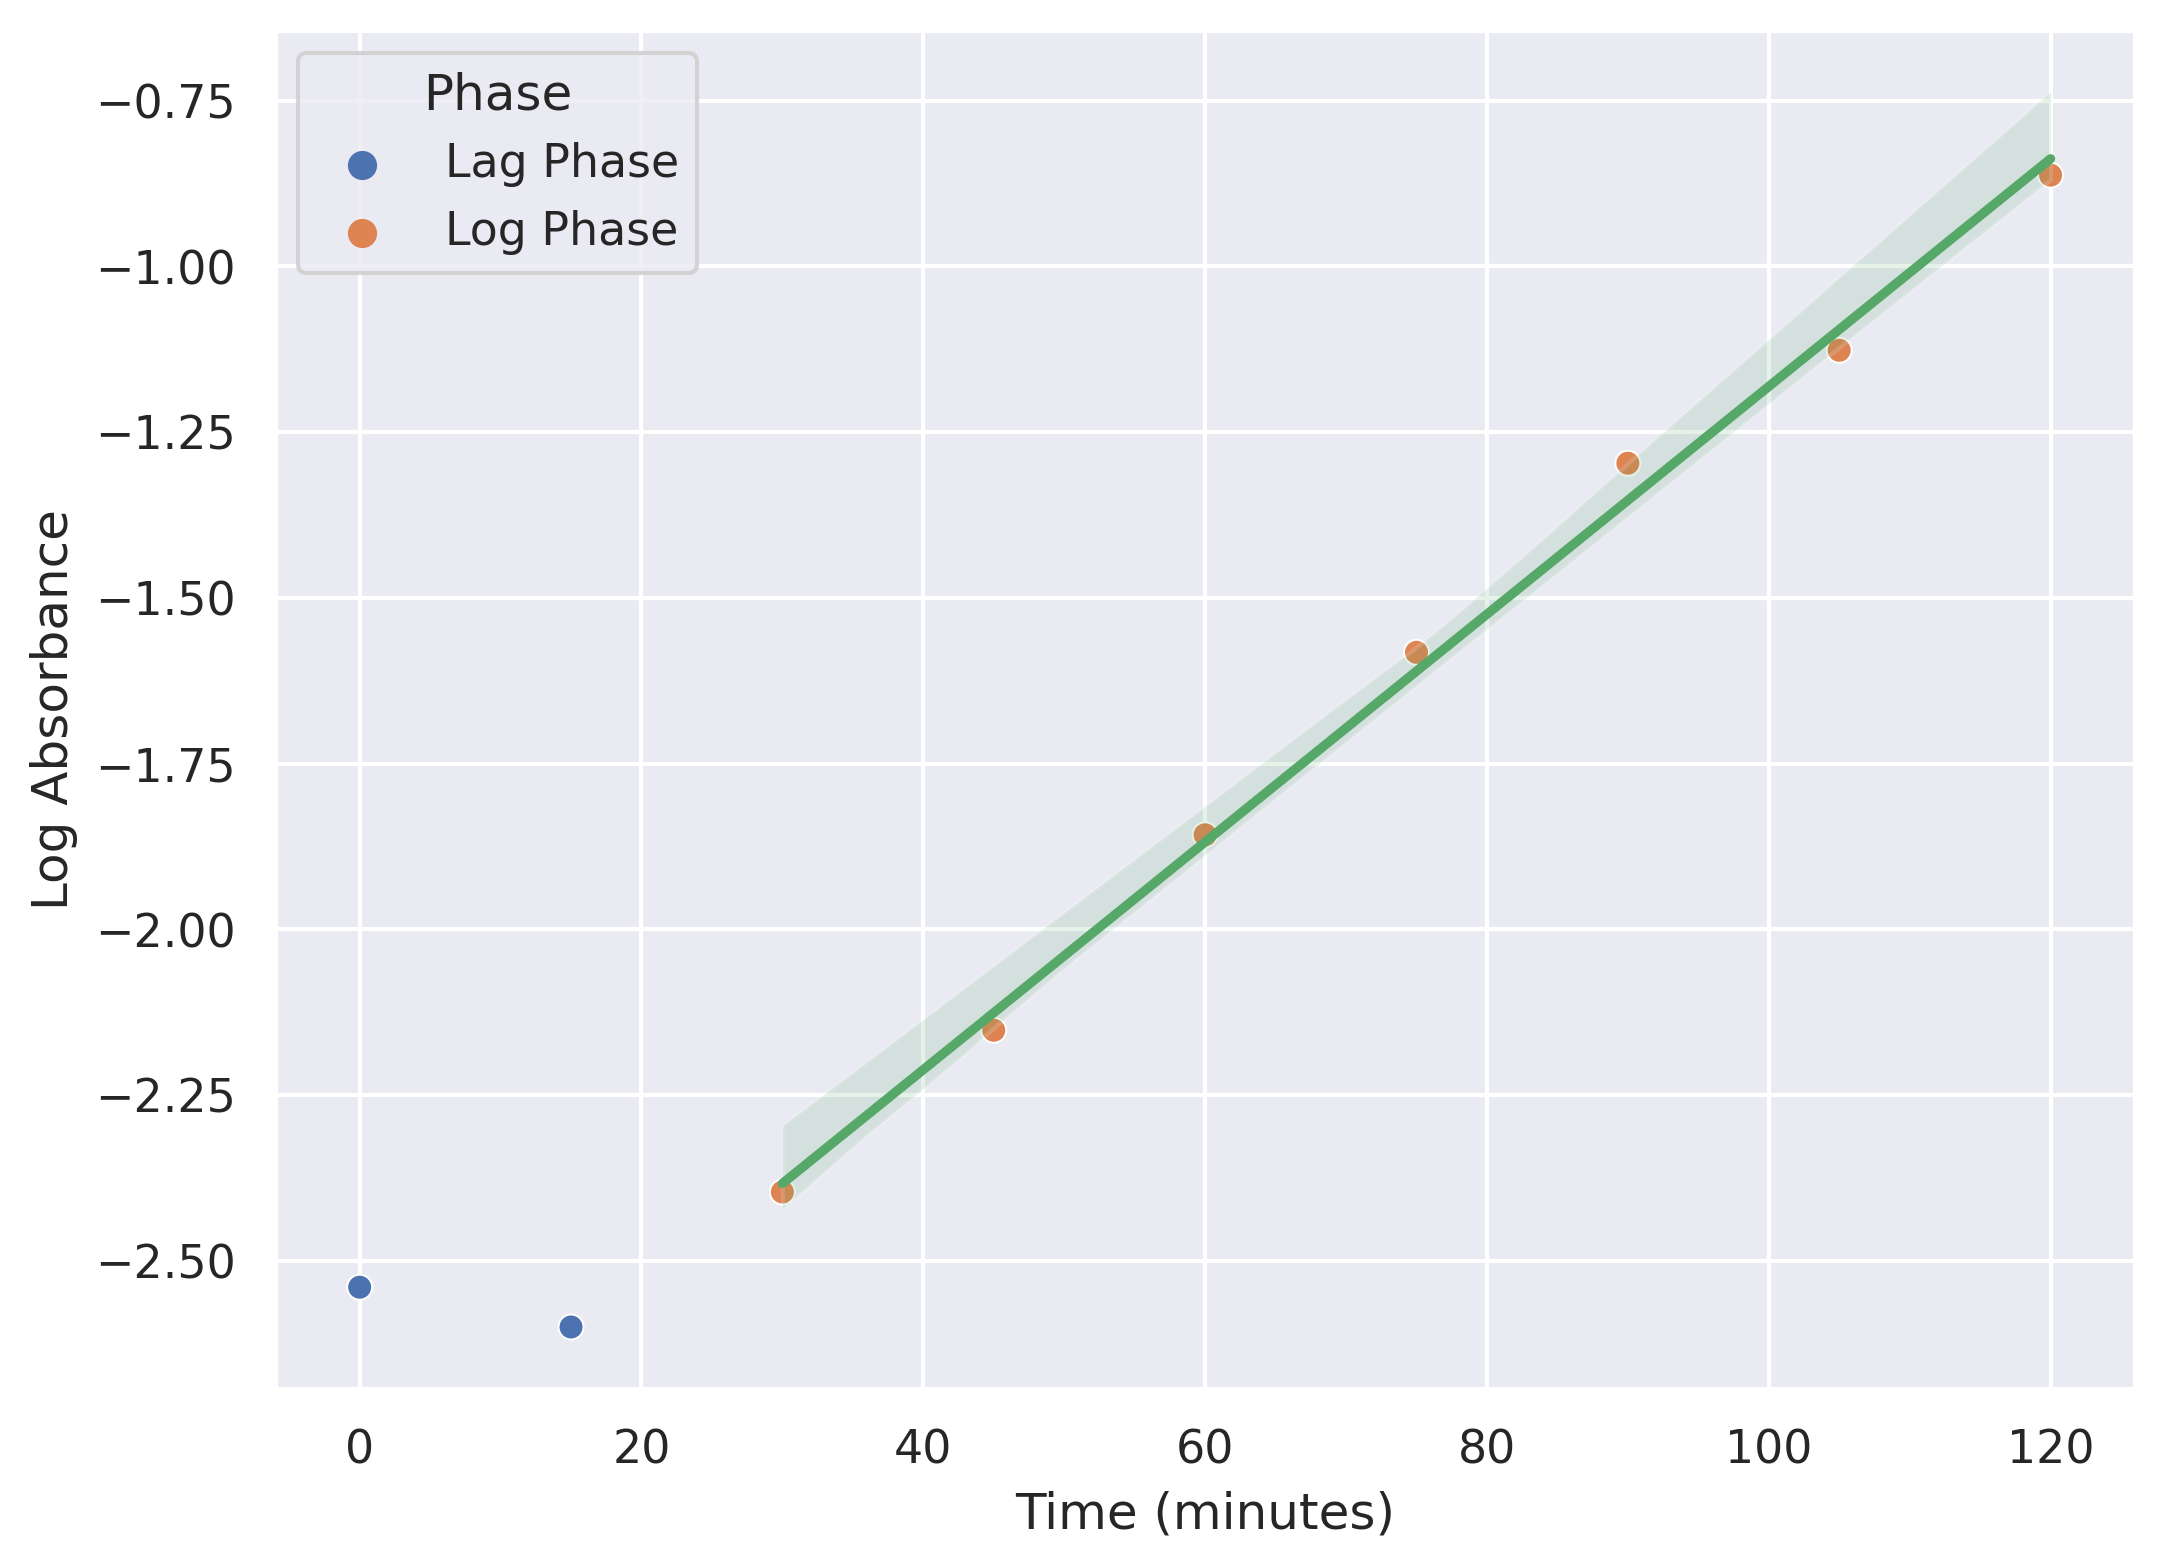
\includegraphics[width=0.9\textwidth]{photos/growth_curve.png}
  \caption{Growth Curve of the Bacterial culture plotted over a 120-minute interval. }\label{fig:growth_curve}
\end{figure}
The equation of the line plotted is \[y = 0.017x - 2.89\]
The following equation was calculated by obtaining two points in the given
straight line and solving the pair of linear equations in two variables (slope
and intercept). A unit increase in the y-axis relates to the doubling of
absorbance. The time taken (increase in the x-axis) for the doubling gives the
\textit{doubling time} of the bacteria. Mathematically, it can be calculated by
taking the inverse of the slope of the line of best fit $\Rightarrow$ 1/0.017 =
\textbf{58.47 minutes}.

\subsection{Calculation of Colony Forming Units}
To obtain information on the concentration of colony-forming units with respect
to the absorbance values, at the 60th-minute interval, the culture was taken
and serially diluted to four concentrations ranging from $10^{-3}$ to
$10^{-6}$. Followingly 100$\mu$L was taken and added to the agar plate for
incubation and then the colonies were visually counted. The following table
summarizes the cfu/100$\mu$L at different dilutions and the calculated cfu/mL
for the bacteria.

\begin{table}[h]
  \begin{center}
    \caption{Colonies counted over different serial dilutions. *Note: 100$\mu$L was added rather than 1mL}\label{tab:colonies}%
    \begin{tabular}{  m{4em}  m{4em} m{4.5em}  m{4.5em}  m{4.5em} m{4.5em}  m{6em} }
      \toprule
      Time (mins)         & A\textsubscript{600}   & Colonies on $10^{-3}$ dilution & Colonies on $10^{-4}$ dilution & Colonies on $10^{-5}$ dilution & Colonies on $10^{-6}$ dilution & Colony forming units per ml (cfu/ml)           \\
      \midrule
      \multirow{4}{*}{60} & \multirow{4}{*}{0.276} & TMTC                           & TMTC                           & $105\pm5$                      & $17\pm1$                       & \multirow{4}{*}{$(121.75\pm25) \times 10^{6}$} \\
                          &                        & TMTC                           & TMTC                           & $121\pm5$                      & $11\pm1$                       &                                                \\
                          &                        & TMTC                           & TMTC                           & $127\pm5$                      & $12\pm1$                       &                                                \\
                          &                        & TMTC                           & TMTC                           & $134\pm5$                      & $14\pm1$                       &                                                \\
      \botrule

    \end{tabular}
  \end{center}
\end{table}

The most optimal measurement was taken at the $10^{-5}$ dilution.

$\Rightarrow$ Average CFU / 100$\mu$L at $10^{-5}$ dilution = $121.75\pm25$.

$\Rightarrow$ CFU / 100$\mu$L at $10^{0}$ dilution = $(121.75\pm25) \times 10^{5}$.

$\Rightarrow$ CFU / 1mL at $10^{0}$ dilution =  $(121.75\pm25) \times 10^{6}$.

\section{Experiment 2}\label{sec:exp2}

\subsection{Mixed Culture Bacteria}\label{subsec:mixed}
\subsubsection{Species Name}
Mixed Culture Bacteria
\subsubsection{Description of Bacteria under the Agar plate}
Bacterial colonies were prominently visible on the agar plate. There were
densely packed regions of bacteria colonies suggesting the presence of cocci
packets alongside sparsely spread bacteria suggesting the presence of
rod-shaped bacteria. The visible number of colonies under the agar plate was in
the order of hundreds.
\subsubsection{Stain Used for Microscopic Analysis}
The procedure was carried out via four subsequent staining steps $\Rightarrow$
Crystal Violet (1 minute), Lugol's Solution (1 minute), Decolorization Solution
(10 seconds), and Safranine Red (1 minute).

\subsubsection{Description of Stained Culture}
\begin{figure}[h]%
  \centering
  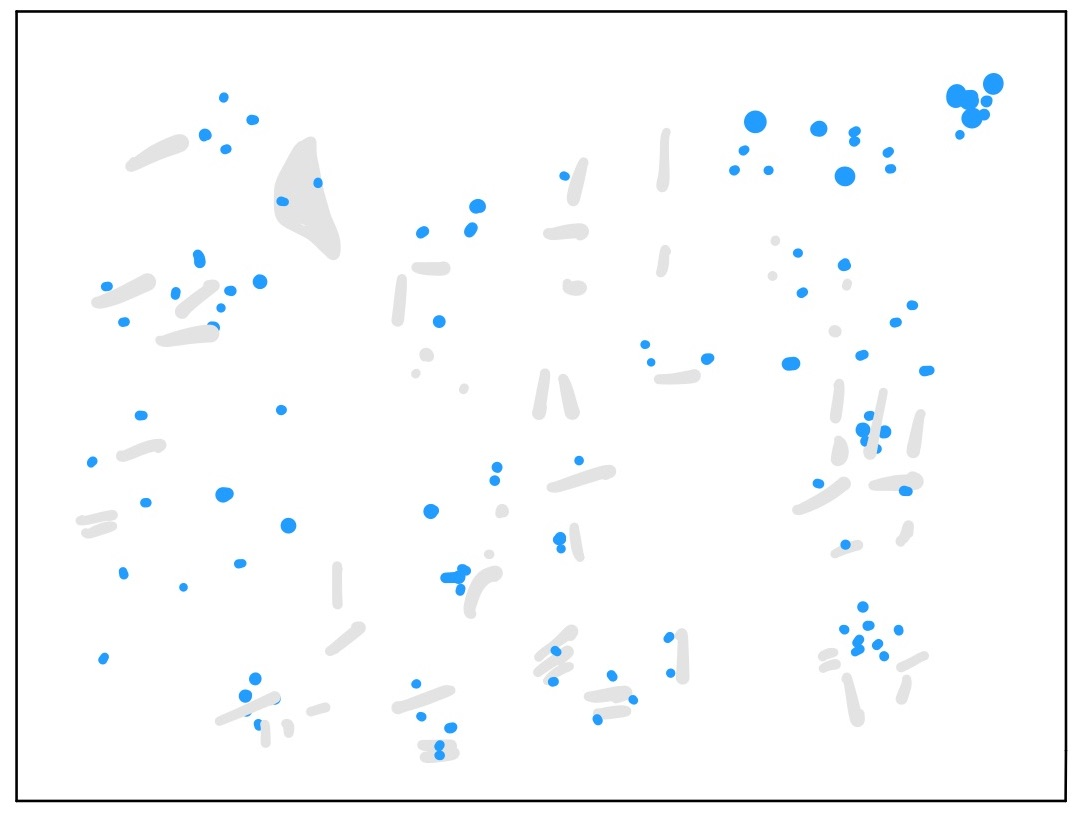
\includegraphics[width=0.6\textwidth]{photos/MC.jpg}
  \caption{The following drawing depicts the visual attributes of Mixed Stained bacteria viewed under 100x zoom. }\label{fig:mixed}
\end{figure}

A mixture of two species of colored bacteria could be observed $\Rightarrow$
\begin{itemize}
  \item The first species is brightly violet-colored and cocci shaped. The cells are
        randomly spaced and do seem to form big chains or clusters. They are however
        relatively close together than rod-shaped bacteria. The size of these bacteria
        is almost identical.
  \item The second species is a dark pink colored rod-shaped bacteria. It is more
        sparsely distanced than the former and tends to have some angled arrangement as
        well as pair-wise occurrence.
\end{itemize}

\subsubsection{Conclusion}
According to the visual characteristics observed, the first species seems to be
a gram-positive cocci bacteria that occurs in packets. The second species seems
to be either a randomly sparsed or angled-arrangement gram-negative bacillus.

\subsection{Bacterial Culture A}\label{subsec:culture_a}
\subsubsection{Species Name}
\textit{Escherichia Coli}.
\subsubsection{Description of Bacteria under the Agar plate}
Bacterial colonies were prominently visible on the agar plate. The colonies
appeared to be smooth, circular, and randomly dispersed throughout the agar.
\subsubsection{Stain Used for Microscopic Analysis}
The procedure was carried out via four subsequent staining steps $\Rightarrow$
Crystal Violet (1 minute), Lugol's Solution (1 minute), Decolorization Solution
(10 seconds), and Safranine Red (1 minute).

\subsubsection{Description of Stained Culture}
\begin{figure}[h]%
  \centering
  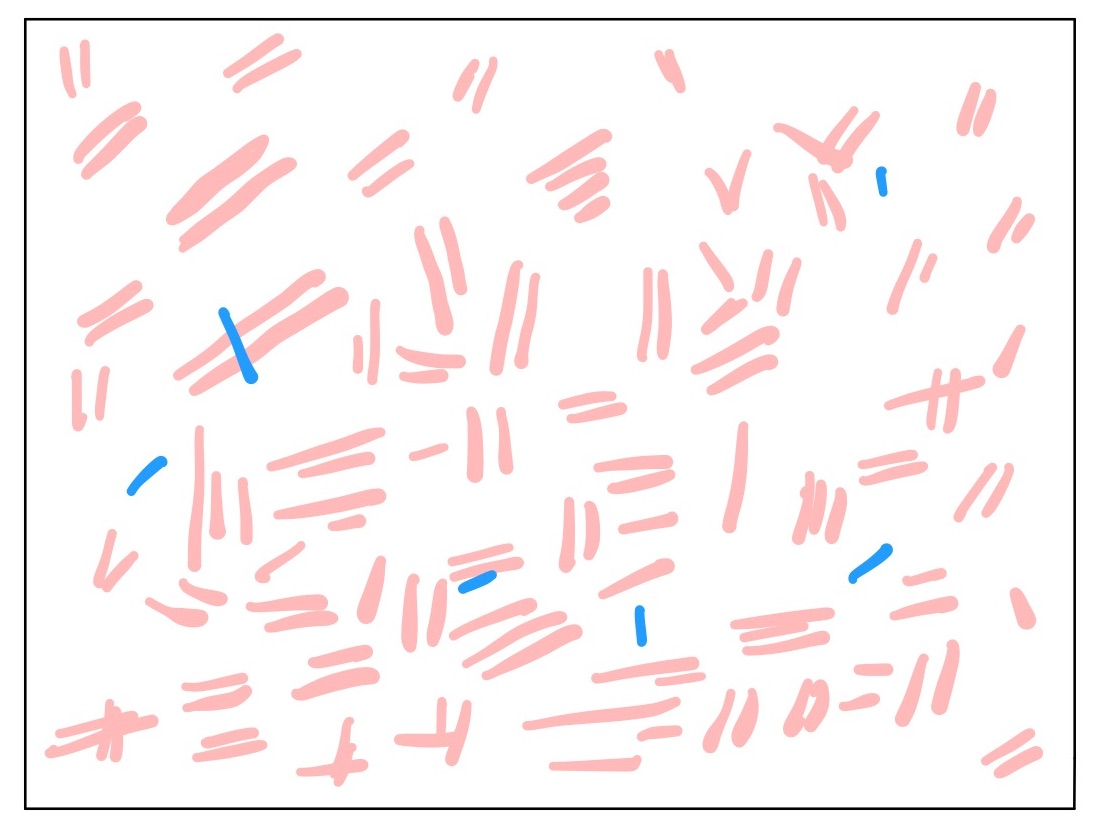
\includegraphics[width=0.6\textwidth]{photos/A.jpg}
  \caption{The following drawing depicts the visual attributes of Bacterial Culture A viewed under 100x zoom. }\label{fig:culture_a}
\end{figure}

\begin{itemize}
  \item The bacterial colonies appear to be rod-shaped and pinkish in color with a few
        notable violet-stained bacteria that could be the result of contamination.
  \item The cells seemed to have densely occupied the entire slide.
  \item There is no chain formation or visible clustering. The arrangement is almost
        random.
\end{itemize}

\subsubsection{Conclusion}
It can clearly be verified that the absence of blue/violet stain indicates that
the bacteria present is gram-negative which in fact is true with \textit{E.
  Coli}.

\subsection{Bacterial Culture C}\label{subsec:culture_c}
\subsubsection{Species Name}
\textit{Bacillus subtilis}.
\subsubsection{Description of Bacteria under the Agar plate}
Bacterial colonies were prominently visible on the agar plate. The colonies
appeared to be yellowish-white colored, smooth, circular, shiny, and randomly
dispersed throughout the agar.
\subsubsection{Stain Used for Microscopic Analysis}
Schaeffer \& Fulton's method was followed for staining with Malachite Green.

\subsubsection{Description of Stained Culture}
\begin{figure}[h]%
  \centering
  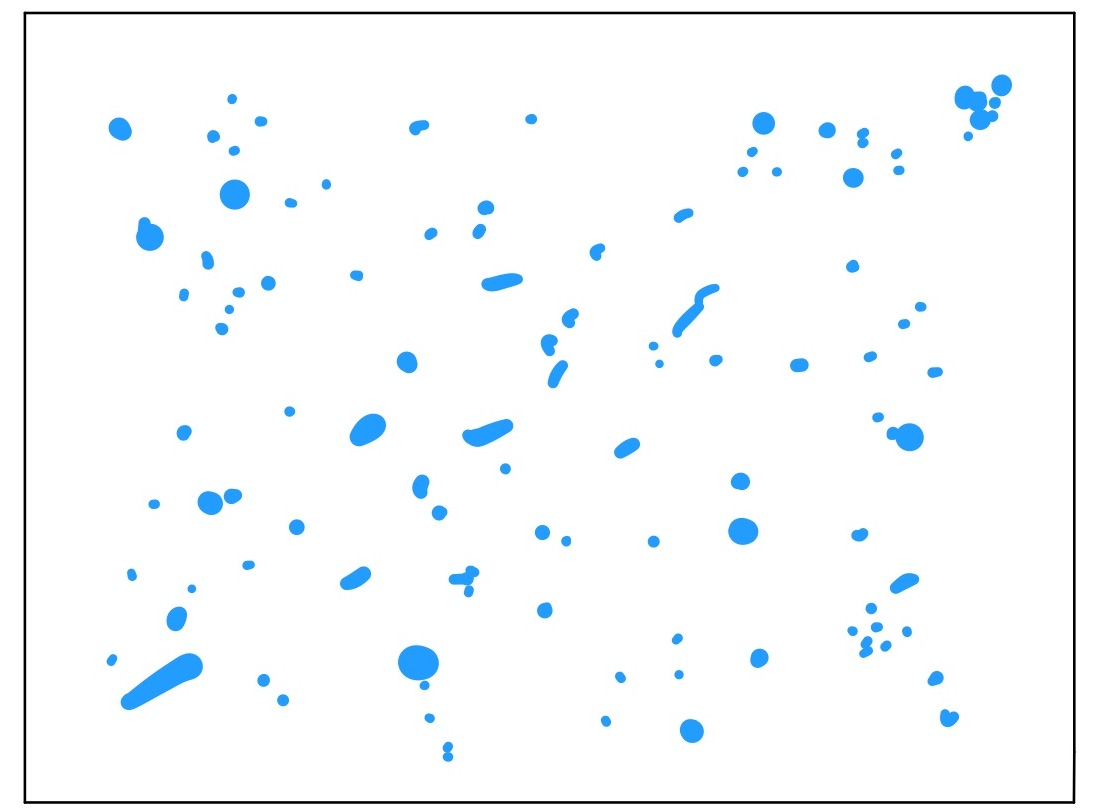
\includegraphics[width=0.6\textwidth]{photos/C.jpg}
  \caption{The following drawing depicts the visual attributes of Bacterial Culture C viewed under 100x zoom. }\label{fig:culture_c}
\end{figure}

\begin{itemize}
  \item The bacterial colonies appear mostly to be bacilli-shaped and violet in color.
        There are cells however of different shapes that could be visible.
  \item These different shapes could possibly indicate the spore formation on the
        bacteria or possible clustering.
  \item Relative to the bacilli slide, these bacteria are more sparsely distanced.
\end{itemize}

\subsubsection{Conclusion}
It can clearly be verified that the presence of blue/violet color alongside
spore-like features in some cells indicates that the bacteria present is a
gram-positive sporulating culture which in fact is true with \textit{Bacillus
  subtilis}.

\subsection{Sources of Error}\label{subsec:errors}
\begin{enumerate}
  \item One of the most prominent sources of error is the contamination of the glass
        slides while transferring the bacteria.
  \item Subsequently, as the bacteria within the colonies are densely packed making
        them highly sensitive to the quantity of bacteria taken from the agar plate. If
        an excess of bacteria is taken into the slide, the microscopic image would be
        heavily layered and make it difficult to distinguish visual traits.
  \item The quintessential factor in viewing bacterial cultures under the microscope is
        the proper incubation of bacteria. If the incubation is carried out
        incorrectly, experimental results might be obtained incorrectly or even not at
        all.
\end{enumerate}

\end{document}
